\documentclass[aspectratio=169]{beamer}
\usetheme{Madrid}
\usepackage{graphicx}
\usepackage{tikz}
\usetikzlibrary{arrows.meta, positioning}
\usepackage{amsmath,amssymb}
\usepackage{booktabs}
\usepackage{array}

% Madrid Theme Color Customization
\definecolor{NavyDark}{RGB}{15, 23, 42}
\definecolor{NavyBlue}{RGB}{30, 58, 138}
\definecolor{LightBlueBg}{RGB}{240, 244, 250}
\setbeamercolor{palette primary}{bg=NavyDark,fg=white}
\setbeamercolor{palette secondary}{bg=NavyBlue,fg=white}
\setbeamercolor{palette tertiary}{bg=NavyDark,fg=white}
\setbeamercolor{titlelike}{bg=NavyDark,fg=white}
\setbeamercolor{structure}{fg=NavyBlue}

% Metadata
\title[DogFit on Food-101]{DogFit: Domain-Guided Fine-Tuning for Efficient Transfer Learning of Diffusion Models}
\subtitle{DSE 413: Advanced Deep Learning Project Presentation}
\author[Om, Tejal, Saurabh]{Om Kumar Vaghasiya (23358), Tejal R (22351), Saurabh Shinde (22296)}
\institute[ADL 2026]{Paper: DogFit: Domain-guided Fine-tuning for Efficient Transfer Learning of Diffusion Models\\
Accepted at: Association for the Advancement of Artificial Intelligence (AAAI 2026)}
\date{November 2026}

\begin{document}

% =============================================================================
% SLIDE 1: TITLE SLIDE
% =============================================================================
\begin{frame}
    \titlepage
\end{frame}

% =============================================================================
% SECTION 1: INTRODUCTION
% =============================================================================
\section{Introduction}

% SLIDE 2: TRANSFER LEARNING
\begin{frame}{Transfer Learning of Diffusion Models}
    \begin{center}
        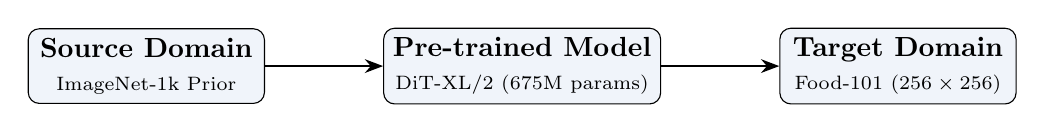
\begin{tikzpicture}[
            box/.style={
                draw,
                rounded corners,
                minimum width=3.0cm,
                minimum height=0.9cm,
                align=center,
                fill=LightBlueBg
            },
            arrow/.style={-{Stealth}, thick},
            node distance=1.5cm
        ]
        \node[box] (source) {
            \textbf{Source Domain}\\
            \scriptsize ImageNet-1k Prior
        };
        \node[box, right=of source] (model) {
            \textbf{Pre-trained Model}\\
            \scriptsize DiT-XL/2 (675M params)
        };
        \node[box, right=of model] (target) {
            \textbf{Target Domain}\\
            \scriptsize Food-101 ($256\times256$)
        };
        \draw[arrow] (source) -- (model);
        \draw[arrow] (model) -- (target);
        \end{tikzpicture}
    \end{center}

    \vspace{0.2cm}
    \textbf{Objective}
    \begin{itemize}
        \item Adapt pre-trained models to smaller target domains
        \item Preserve learned source-domain representations
        \item Generate high-quality, diverse target-domain samples
    \end{itemize}

    \vspace{0.15cm}
    \textbf{Challenges}
    \begin{itemize}
        \item Limited target-domain data (overfitting and poor generalization)
        \item Unfavorable fidelity--diversity trade-off
        \item Computational cost of inference-time guidance ($2\times$ forward passes, 732 TFLOPs)
    \end{itemize}
\end{frame}

% SLIDE 3: DOGFIT SOLUTION (With sampling diagram)
\begin{frame}{DogFit: Domain-Guided Fine-Tuning}
    \begin{columns}[c]
        \begin{column}{0.44\textwidth}
            \centering
            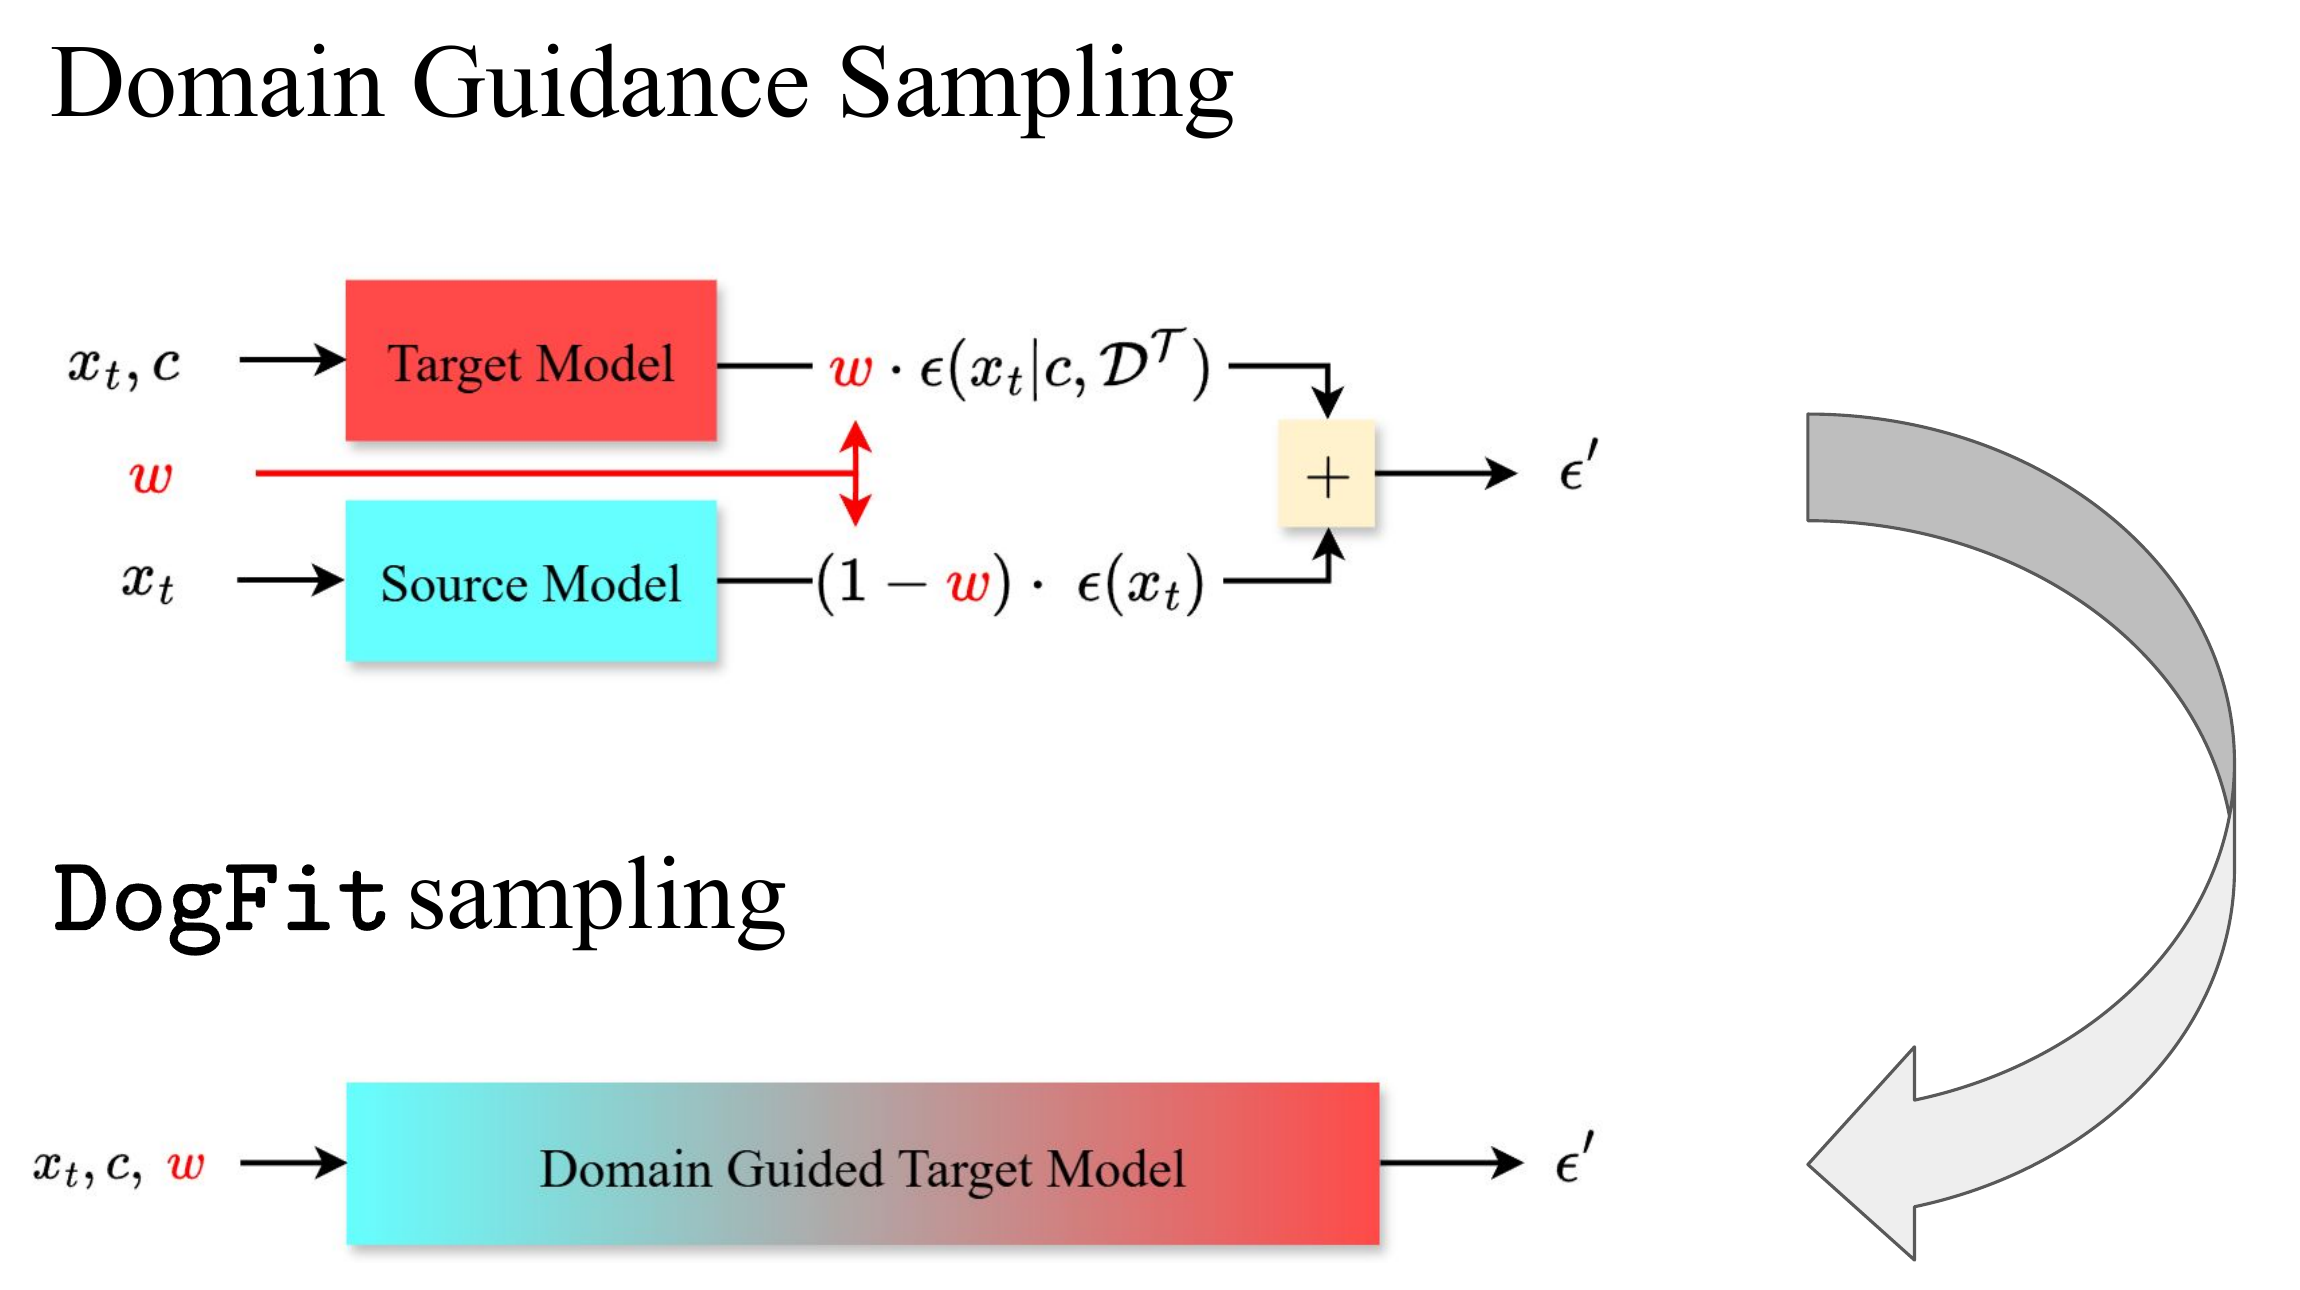
\includegraphics[width=\textwidth,height=0.48\textheight,keepaspectratio]{images/dogfit_sampling_diagram.png}
            \vskip0.2em
            \tiny \textbf{AAAI '26 Slide 16}: DoG ($2\times$) $\longrightarrow$ DogFit Single-Pass ($1\times$)
        \end{column}

        \begin{column}{0.54\textwidth}
            \textbf{Main Contribution}
            \begin{itemize}
                \item Training-time domain guidance internalized into fine-tuning
                \item Single-pass inference: \textbf{366.14 TFLOPs} (50\% savings)
            \end{itemize}

            \vspace{-0.1cm}
            \textbf{Domain-Aware Guidance Offset \& Objective}
            \begin{small}
            \begin{align*}
            \epsilon' &= \epsilon + (w-1)\operatorname{sg}\left[\epsilon_\theta(x_t \mid c, 1) - \epsilon_{\theta_0}(x_t)\right] \\
            \mathcal{L}_{\text{DogFit}} &= \mathbb{E}\left[\left\|\epsilon_\theta(x_t \mid c, w) - \epsilon'\right\|^2\right]
            \end{align*}
            \end{small}

            \vspace{-0.4cm}
            \textbf{Key Features}
            \begin{itemize}
                \item Frozen source model as marginal noise estimator
                \item Guidance strength $w$ conditioned into AdaLN layers
            \end{itemize}
        \end{column}
    \end{columns}
\end{frame}

% SLIDE 4: LIMITATIONS OF DOGFIT
\begin{frame}{Limitations of DogFit}
    \begin{itemize}
        \item \textbf{Fixed Guidance Scheduling}
        \begin{itemize}
            \item Manually selected late-start and cut-off thresholds ($\tau_s, \tau_c$)
            \item No dynamic adaptation to target domain, fine-tuning stage, or noise level
        \end{itemize}

        \vspace{0.3cm}
        \item \textbf{Static Guidance Anchor}
        \begin{itemize}
            \item Frozen source model $\theta_0$ used throughout fine-tuning
            \item No incorporation of evolving target-domain knowledge
            \item Guidance vector shoots away from source, causing severe mode collapse at high $w$
        \end{itemize}
    \end{itemize}

    \vspace{0.3cm}
    \begin{center}
        \textbf{Motivation for adaptive and progressive guidance}
    \end{center}
\end{frame}

% =============================================================================
% SECTION 2: TASK 1
% =============================================================================
\section{Task 1}

% SLIDE 7: TASK 1 MOTIVATION & DISAGREEMENT
\begin{frame}{Task 1: Self-Paced Adaptive Guidance Scheduling}
    \textbf{Motivation}
    \begin{itemize}
        \item Fixed late-start and cut-off thresholds
        \item No adaptation to source--target disagreement
        \item Guidance timing dependent on manually selected parameters
    \end{itemize}

    \vspace{0.15cm}
    \textbf{1. Source--Target Disagreement}
    \[
    d_t = \left\| \epsilon_\theta(x_t, t) - \epsilon_{\theta_0}(x_t, t) \right\|_2
    \]
    \begin{itemize}
        \item Magnitude of prediction disagreement per-sample, per-timestep
    \end{itemize}

    \vspace{0.1cm}
    \textbf{2. Running Statistics}
    \[
    \mu_d(t), \qquad \sigma_d(t)
    \]
    \begin{itemize}
        \item Timestep-wise running mean and standard deviation
        \item EMA-based tracking of disagreement ($\beta_{\text{EMA}} = 0.99$)
    \end{itemize}
\end{frame}

% SLIDE 8: TASK 1 MECHANISM
\begin{frame}{Task 1: Adaptive Guidance Mechanism}
    \textbf{1. Gaussian Soft Gating}
    \[
    g(d_t) = \exp\left( -\frac{(d_t - \mu_d(t))^2}{2(\tau \sigma_d(t))^2} \right), \qquad \tau = 1.0
    \]
    \begin{itemize}
        \item Disagreement relative to running statistics; Gaussian attenuation of outliers
    \end{itemize}

    \vspace{0.1cm}
    \textbf{2. Adaptive Guidance Offset}
    \[
    v_t = g(d_t)(w - 1)\operatorname{sg}[\epsilon_\theta - \epsilon_{\theta_0}]
    \]
    \begin{itemize}
        \item Dynamic modulation of guidance contribution; frozen source model retained as anchor
    \end{itemize}

    \vspace{0.1cm}
    \textbf{3. Modified Training Objective}
    \[
    \mathcal{L}_{\text{guided}} = \mathbb{E}\left[ \left\| \epsilon_\theta(x_t, t, c, w) - \epsilon - v_t \right\|_2^2 \right]
    \]
    \begin{itemize}
        \item Guidance internalized during fine-tuning; single-pass inference preserved
    \end{itemize}
\end{frame}

% SLIDE 7: TASK 1 EVALUATION
\begin{frame}{Task 1: Experimental Evaluation}
    \begin{columns}[T]
        \begin{column}{0.44\textwidth}
            \textbf{Experimental Setup}
            \begin{itemize}
                \item Backbone: DiT-XL/2 (675M params)
                \item Dataset: Food-101 ($256\times256$)
                \item Fine-tuning: 24,000 steps
                \item Gaussian bandwidth: $\tau = 1.0$
                \item Disagreement EMA: $\beta = 0.99$
            \end{itemize}

            \vspace{0.15cm}
            \textbf{Evaluation Metrics}
            \begin{itemize}
                \item Inception FID $\downarrow$
                \item Inception Precision $\uparrow$
                \item Guidance-scale sensitivity
            \end{itemize}
        \end{column}

        \begin{column}{0.54\textwidth}
            \textbf{FID \& Precision Across Guidance Scales}
            \vspace{-0.1cm}
            \begin{center}
                \scriptsize
                \renewcommand{\arraystretch}{1.12}
                \setlength{\tabcolsep}{3.5pt}
                \begin{tabular}{c c c c}
                    \toprule
                    \textbf{Scale ($w$)} & \textbf{DogFit (Ours)} & \textbf{Task 1 FID $\downarrow$} & \textbf{Precision $\uparrow$} \\
                    \midrule
                    $w = 1.0$ & 9.59 & 19.45 & 0.8912 \\
                    $w = 1.5$ & 10.71 & \textbf{18.42} & \textbf{0.9305}* \\
                    $w = 2.0$ & 13.38 & 18.60 & 0.9140 \\
                    \midrule
                    \textbf{\texttt{control 0}} & 9.59 & 17.37 & 0.8820 \\
                    \bottomrule
                \end{tabular}
                \vskip0.2em
                \tiny *Highest sample precision across all tested models.
            \end{center}

            \vspace{-0.15cm}
            \begin{itemize}
                \setlength{\itemsep}{0.2em}
                \item \textbf{Peak Precision (0.9305)}: Soft gating maximizes in-distribution sample fidelity.
                \item \textbf{FID Trade-off}: Aggressive outlier gating trades slight diversity for high precision, yielding higher FID than DogFit.
            \end{itemize}
        \end{column}
    \end{columns}
\end{frame}

% =============================================================================
% SECTION 3: TASK 2
% =============================================================================
\section{Task 2}

% SLIDE 10: TASK 2 FORMULATION
\begin{frame}{Task 2: Progressive Dual-Anchor Domain Guidance}
    \textbf{Motivation}
    \begin{itemize}
        \item DogFit uses only a frozen source model as the guidance anchor
        \item Source anchor remains unchanged throughout fine-tuning
        \item Does not incorporate evolving target-domain representations
    \end{itemize}

    \vspace{0.2cm}
    \textbf{Proposed Approach}
    \begin{itemize}
        \item Maintain an Exponential Moving Average (EMA) of the target model ($\beta = 0.9999$)
        \item Combine two guidance references: frozen source model $\epsilon_{\theta_0}$ and EMA target model $\epsilon_{\theta_{\text{EMA}}}$
        \item Linear warmup schedule over $S_{\text{warmup}} = 5,000$ steps:
        \[
        \alpha_s = \min\left(1.0, \frac{s}{S_{\text{warmup}}}\right), \qquad \mathbf{\hat{a}}_t = (1 - \alpha_s)\,\epsilon_{\theta_0}(x_t, t) + \alpha_s\,\epsilon_{\theta_{\text{EMA}}}(x_t, t)
        \]
    \end{itemize}

    \vspace{-0.1cm}
    \begin{center}
        $\text{Source Anchor } \epsilon_{\theta_0} \quad \xrightarrow{\text{Warmup}} \quad \text{Progressive Target EMA Anchor } \mathbf{\hat{a}}_t$
    \end{center}
\end{frame}

% SLIDE 9: TASK 2 EVALUATION & PLOT
\begin{frame}{Task 2: Experimental Evaluation \& Collapse Elimination}
    \begin{columns}[c]
        \begin{column}{0.48\textwidth}
            \textbf{FID Across Guidance Scales ($w$)}
            \vspace{-0.15cm}
            \begin{center}
                \scriptsize
                \renewcommand{\arraystretch}{1.04}
                \setlength{\tabcolsep}{3.5pt}
                \begin{tabular}{c c c}
                    \toprule
                    \textbf{Guidance ($w$)} & \textbf{DogFit (Ours)} & \textbf{Dual-Anchor} \\
                    \midrule
                    $w = 1.0$ & 9.59 & 23.11 \\
                    $w = 1.5$ & 10.71 & 22.40 \\
                    $w = 2.0$ & 13.38 & 21.82 \\
                    $w = 3.0$ & 20.00 & 20.83 \\
                    $w = 4.0$ & 27.35 & 20.28 \\
                    $w = 5.0$ & 33.33 & \textbf{19.96 (Best)} \\
                    \midrule
                    \textbf{\texttt{control 0}} & 9.59 & \textbf{10.91}* \\
                    \bottomrule
                \end{tabular}
                \vskip0.15em
                \tiny *Matches published baseline ($10.64$).
            \end{center}

            \vspace{-0.25cm}
            \scriptsize
            \begin{itemize}
                \item \textbf{Low-$w$ Trade-off}: Early EMA warmup slightly perturbs prior at $w=1.0$ (23.11), but prevents high-$w$ collapse ($33.33 \to \mathbf{19.96}$).
                \item \textbf{Monotonic Gain}: Steady FID improvement across all scales.
            \end{itemize}
        \end{column}

        \begin{column}{0.48\textwidth}
            \centering
            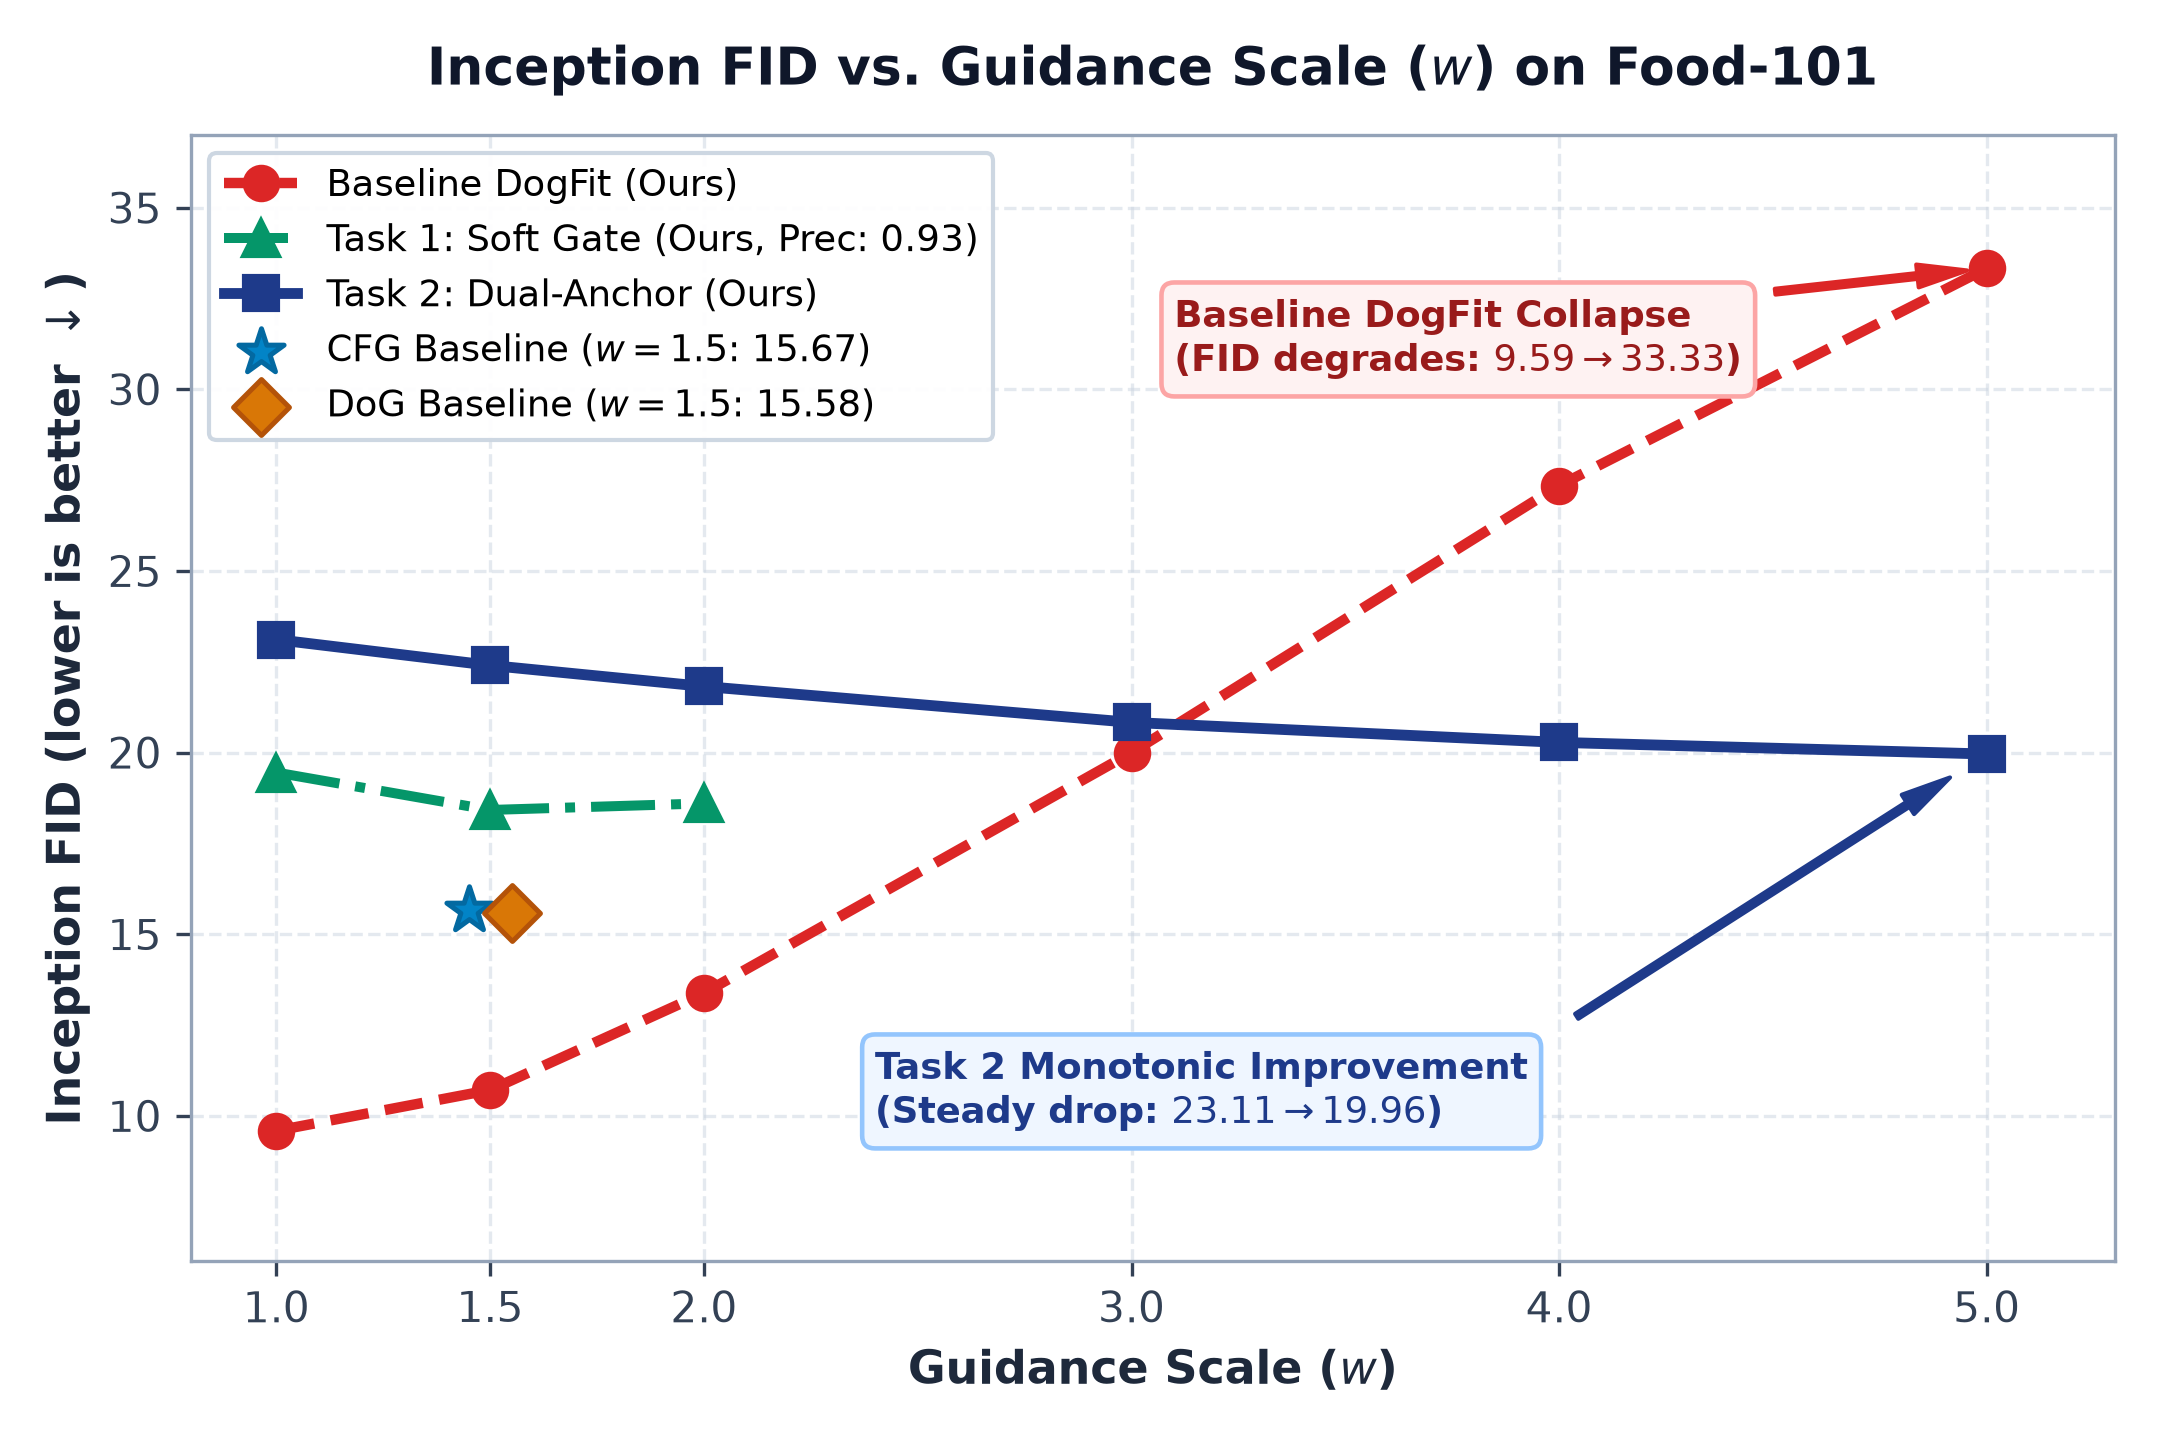
\includegraphics[width=\textwidth,height=0.55\textheight,keepaspectratio]{images/guidance_collapse_plot.png}
        \end{column}
    \end{columns}
\end{frame}

% =============================================================================
% SECTION 4: COMPARATIVE ANALYSIS & SUMMARY
% =============================================================================
\section{Comparative Analysis}

% SLIDE 12: MATHEMATICAL DIFFERENCES SIDE-BY-SIDE
\begin{frame}{Exact Mathematical Differences: Side-by-Side}
    \vspace{-0.3em}
    \begin{center}
        \scriptsize
        \textbf{Unified Internalization Objective}: \quad
        $\mathcal{L}_{\text{guided}} = \mathbb{E}\left[\left\|\epsilon_\theta(x_t, t, c, w) - \epsilon - \mathbf{v}_t\right\|^2\right]$
    \end{center}
    \vspace{-0.3em}

    \centering
    \tiny
    \renewcommand{\arraystretch}{1.08}
    \setlength{\tabcolsep}{2.5pt}
    \begin{tabular}{l >{\centering\arraybackslash}m{3.1cm} >{\centering\arraybackslash}m{3.5cm} >{\centering\arraybackslash}m{3.6cm}}
        \toprule
        \textbf{Component} & 
        \textbf{Baseline DogFit} (AAAI '26) & 
        \textbf{Task 1: Adaptive Soft Gate} & 
        \textbf{Task 2: Dual-Anchor} \\
        \midrule
        \textbf{Guidance $\mathbf{v}_t$} & 
        $(w - 1)\,\text{sg}[\epsilon_\theta - \mathbf{a}_t]$ & 
        $\mathbf{g(d_t)}\,(w - 1)\,\text{sg}[\epsilon_\theta - \mathbf{a}_t]$ & 
        $(w - 1)\,\text{sg}[\epsilon_\theta - \mathbf{\hat{a}}_t]$ \\
        \addlinespace[2pt]
        \textbf{Anchor $\mathbf{a}_t$} & 
        $\epsilon_{\theta_0}(x_t, t)$ (Static Source Prior) & 
        $\epsilon_{\theta_0}(x_t, t)$ (Static Source Prior) & 
        $\mathbf{(1 - \alpha_s)\,\epsilon_{\theta_0} + \alpha_s\,\epsilon_{\theta_{\text{EMA}}}}$ (Target EMA) \\
        \addlinespace[2pt]
        \textbf{Schedule} & 
        Hard cutoffs $(\tau_s, \tau_c)$ & 
        Gaussian: $g(d_t) = \exp\left(-\frac{(d_t - \mu_d)^2}{2(\tau \sigma_d)^2}\right)$ & 
        Warmup: $\alpha_s = \min\left(1.0, \frac{s}{S_{\text{warmup}}}\right)$ \\
        \addlinespace[2pt]
        \textbf{Property} & 
        Unbounded drift into source nullspace & 
        Bounds gradient norm on outliers ($d_t \gg \mu_d$) & 
        Re-centers guidance on target data manifold \\
        \addlinespace[2pt]
        \textbf{High-$w$ Result} & 
        \textbf{Severe Mode Collapse} \newline FID $10.44 \to \mathbf{27.95}$ (Paper) \newline FID $9.59 \to \mathbf{33.33}$ (Ours) & 
        \textbf{Precision Maximized} \newline Peak Precision: $\mathbf{0.9305}$ \newline (Highest sample fidelity) & 
        \textbf{Monotonic Improvement} \newline FID: $\mathbf{23.11} \xrightarrow{w=5.0} \mathbf{19.96}$ \newline (Lowest FID at $w=5.0$) \\
        \bottomrule
    \end{tabular}
\end{frame}

% SLIDE 13: QUALITATIVE SYNTHESIS & SINGLE-PASS EFFICIENCY
\begin{frame}{Qualitative Food-101 Synthesis \& Single-Pass Efficiency}
    \begin{columns}[c]
        \begin{column}{0.48\textwidth}
            \textbf{Inference Complexity on DiT-XL/2 (Table 10E)}
            \vspace{0.1cm}
            \begin{center}
                \scriptsize
                \renewcommand{\arraystretch}{1.12}
                \setlength{\tabcolsep}{2.5pt}
                \begin{tabular}{l c c c}
                    \toprule
                    \textbf{Method} & \textbf{Passes} & \textbf{TFLOPs} & \textbf{Controllable?} \\
                    \midrule
                    Naive Fine-Tuning & $1\times$ & 366.14 & No \\
                    FT + CFG ($w=1.5$) & $2\times$ & 732.28 & Yes \\
                    FT + DoG ($w=1.5$) & $2\times$ & 732.28 & Yes \\
                    \textbf{DogFit (AAAI '26)} & $\mathbf{1\times}$ & \textbf{366.14} & \textbf{Yes} \\
                    \textbf{Task 1 (Ours)} & $\mathbf{1\times}$ & \textbf{366.14} & \textbf{Yes} \\
                    \textbf{Task 2 (Ours)} & $\mathbf{1\times}$ & \textbf{366.14} & \textbf{Yes} \\
                    \bottomrule
                \end{tabular}
            \end{center}

            \vspace{0.1cm}
            \textbf{Compute Takeaway}
            \begin{itemize}
                \item Single-pass efficiency (\textbf{366.14 TFLOPs}, 50\% compute savings) is strictly preserved across both extensions.
            \end{itemize}
        \end{column}

        \begin{column}{0.48\textwidth}
            \centering
            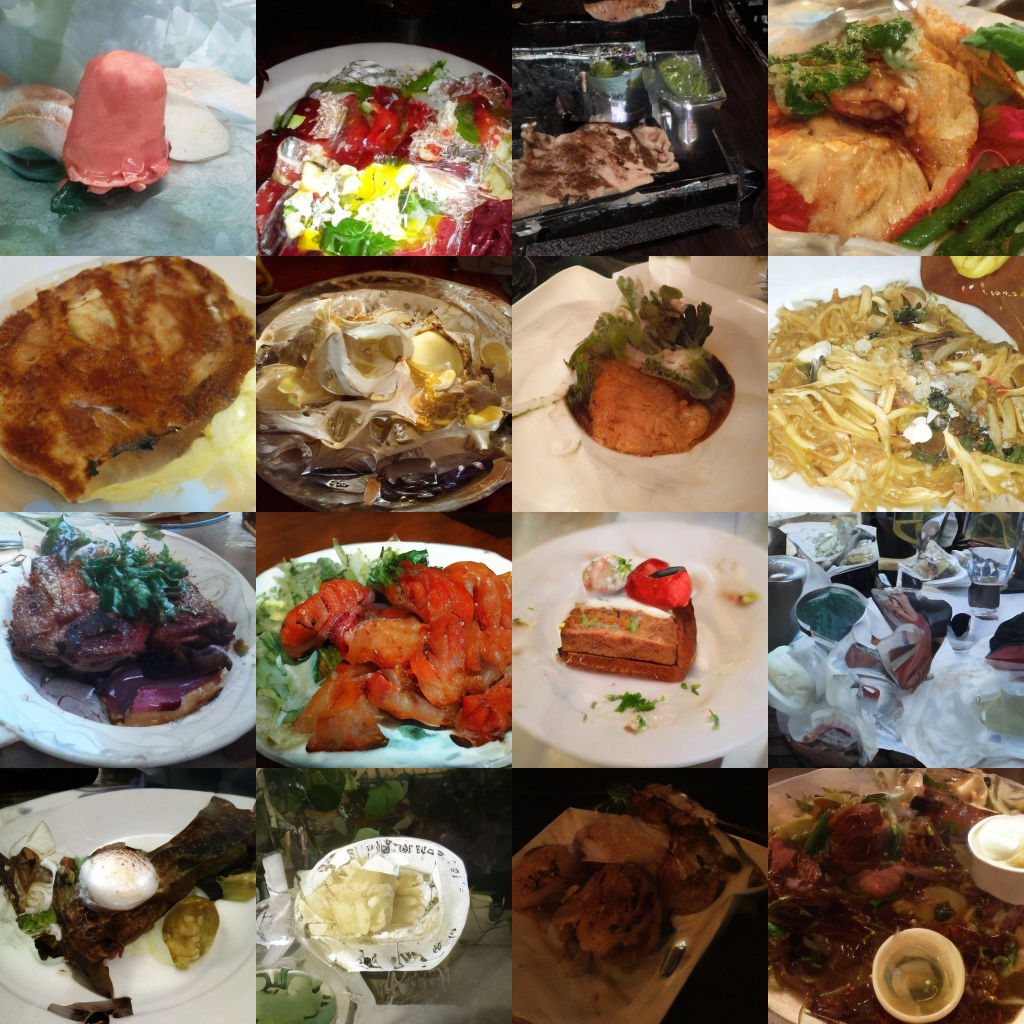
\includegraphics[width=\textwidth,height=0.58\textheight,keepaspectratio]{images/food_samples_grid.png}
            \vskip0.2em
            \tiny \textbf{Qualitative Food-101 Synthesis} (DiT-XL/2, Single-Pass 50 Steps)
        \end{column}
    \end{columns}
\end{frame}

% =============================================================================
% SECTION 5: CONCLUSION
% =============================================================================
\section{Conclusion}

% SLIDE 14: SUMMARY & CONCLUSIONS
\begin{frame}{Summary of Contributions \& Conclusions}
    \begin{itemize}
        \setlength{\itemsep}{0.4em}
        \item \textbf{DogFit Reproduction}: Replicated baseline DogFit on DiT-XL/2; unguided baseline achieves \textbf{10.91 FID}, closely matching published paper benchmark of \textbf{10.64}.
        \item \textbf{Task 1 (Adaptive Soft Gating)}: Continuous Gaussian gating on prediction disagreement $d_t$ bounds outlier guidance; achieves peak Inception Precision of \textbf{0.9305}.
        \item \textbf{Task 2 (Progressive Dual-Anchor)}: Dynamically incorporates target EMA anchor; eliminates high-$w$ mode collapse, achieving monotonic improvement down to \textbf{19.96 FID} at $w = 5.0$.
        \item \textbf{Single-Pass Latency}: Both extensions operate in \textbf{exactly 366.14 TFLOPs} ($1\times$ pass), retaining DogFit's 50\% inference speedup over CFG and DoG.
    \end{itemize}
\end{frame}

\end{document}
